\section{Experimental Results}

% TODO: more details about the setup of experiments

We compared the proposed MACE algorithm with several state-of-the-art parallel Bayesian optimization methods, including the BLCB algorithm\footnote{We implemented this algorithm, as the available open source implementation only takes discrete input}, the local penalization method with EI acquisition function\footnote{Code downloade from https://github.com/SheffieldML/GPyOpt}, the qKG and qEI method\footnote{The code for qKG and qEI is available at https://github.com/wujian16/Cornell-MOE}. The MACE algorithm and the BLCB algorithm are implemented using c++ language. 

\subsection{Benchmark Problems}

We tested the MACE algorithm and other parallel BO method using seven benchmark
functions, including the branin function, the alpine1 function, the 6D hartmann
function, the 2D and 10D ackley function and the 2D and 10D Rosenbrock
function. The dimensions and design space are summarized in Table~ref{tab:summaryanalygical}.

% \begin{table}[htbp]
%     \small
%     \centering
%     \caption{Summary of the analytical benchmark functions}
%     \label{tab:summaryanalygical}
%     \begin{tabular}
%         \toprule
%         Function     & Dimension    & SearchDomain         \\ 
%         \midrule
%         Branin       & 2            & $[-5, 10]\times[0, 15]$ \\
%         Alpine1      & 5            & $[-10, 10]^5$           \\
%         Hartmann6    & 6            & $[0, 1]^6$              \\
%         Ackley2      & 2            & $[-32, 32]^2$           \\
%         Ackley10     & 10           & $[-32, 32]^10$          \\
%         Rosenbrock2  & 2            & $[-5, 10]^2$            \\
%         Rosenbrock10 & 10           & $[-20, 20]^10$          \\
%         \bottomrule
%     \end{tabular}
% \end{table}

\begin{table}[htbp]
    \centering
    \caption{Summary of the analytical benchmark functions}
    \label{tab:summaryanalygical}
    \begin{tabular}{llllllll}
        \toprule
        Function            & Dimension        & Search domain    \\ \midrule
         Branin             & 2                & $[-5, 10]\times[0, 15]$ \\
         Alpine1            & 5                & $[-10, 10]^5$           \\
         Hartmann6          & 6                & $[0, 1]^6$              \\
         Ackley2            & 2                & $[-32, 32]^2$           \\
         Ackley10           & 10               & $[-32, 32]^{10}$          \\
         Rosenbrock2        & 2                & $[-5, 10]^2$            \\
         Rosenbrock10       & 10               & $[-20, 20]^{10}$          \\
        \bottomrule
    \end{tabular}
\end{table}

\begin{enumerate}
        \item Branin
        \item Alpine1
        \item Hart6
        \item Rosenbrock-2
        \item Rosenbrock-10
        \item Ackley-2
        \item Ackley-10
\end{enumerate}

\subsection{Operational Amplifier}

\textcolor{red}{TODO: qKG and qEI}

\begin{figure}[htbp]
\vskip 0.2in
\begin{center}
\centerline{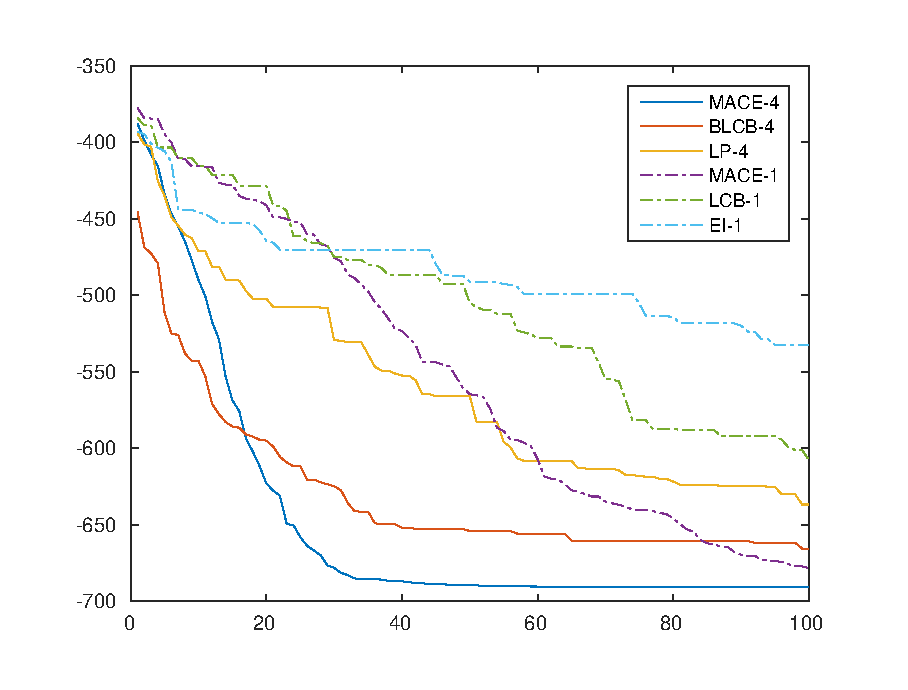
\includegraphics[width=\columnwidth]{./img/mean_DAC2014.eps}}
\caption{Optimization results of the operational amplifier}
\label{resDAC2014}
\end{center}
\vskip -0.2in
\end{figure}


\subsection{ClassE Power Amplifier}

\textcolor{red}{TODO: qKG and qEI}

\begin{figure}[htbp]
\vskip 0.2in
\begin{center}
\centerline{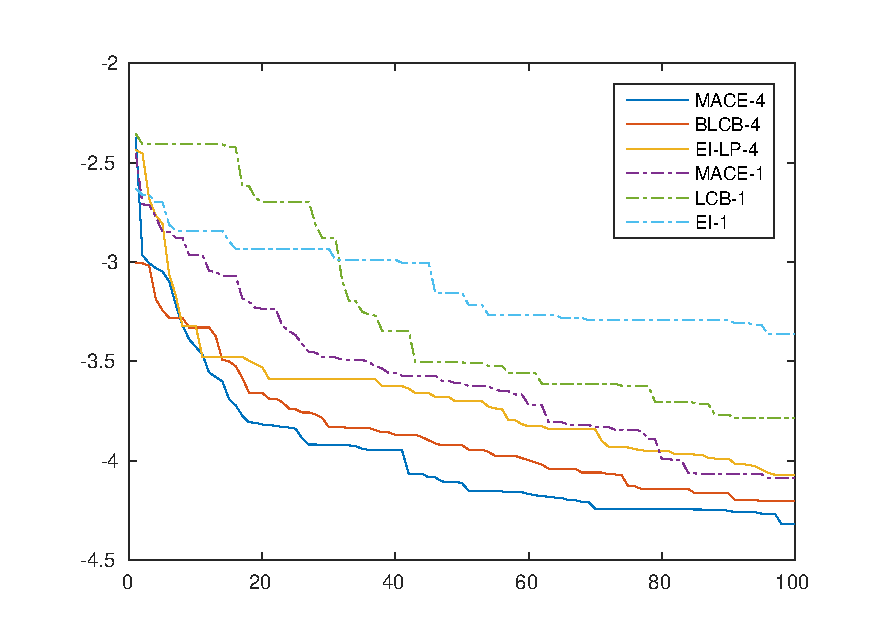
\includegraphics[width=\columnwidth]{./img/ClassE_mean.eps}}
\caption{Optimization results of the class-E power amplifier}
\label{resDAC2014}
\end{center}
\vskip -0.2in
\end{figure}

